
\begin{figure*}[t]
    \centering
    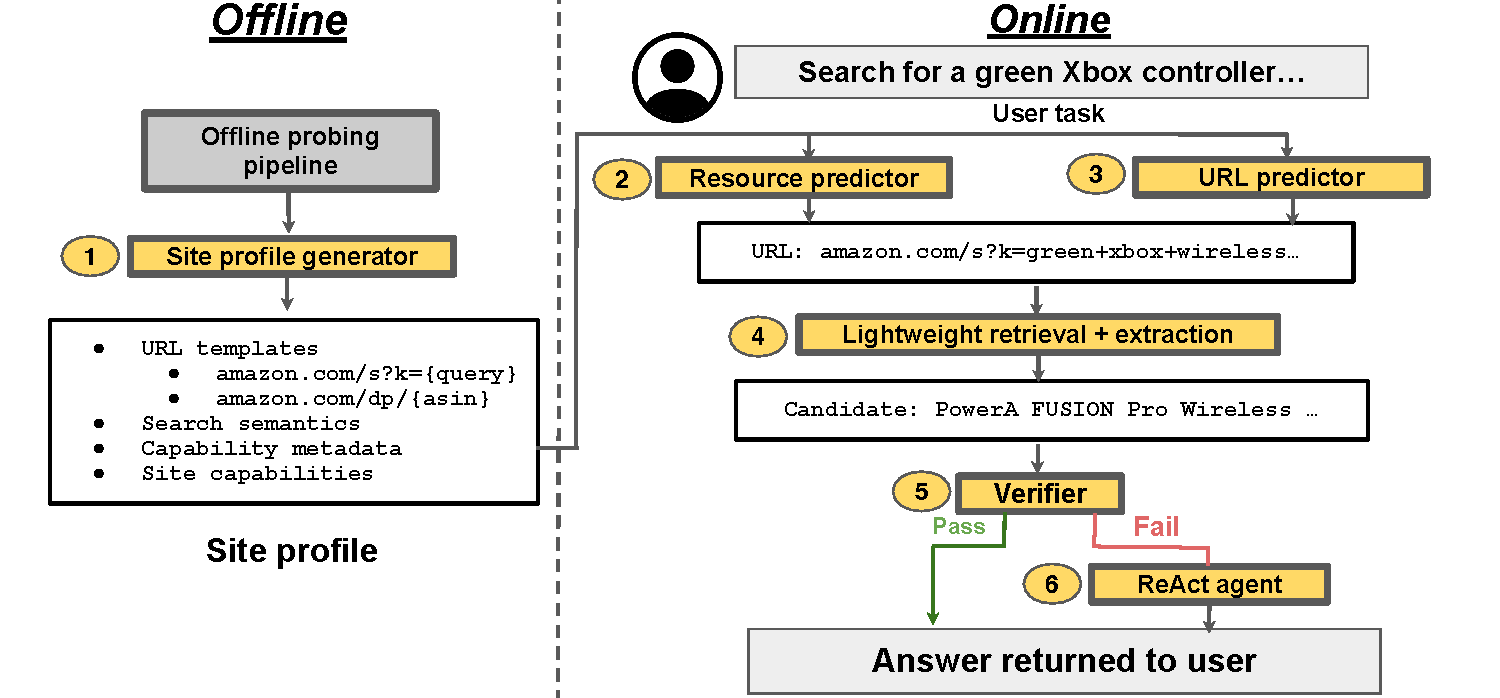
\includegraphics[width=0.8\textwidth]{figures/web-agent-workflow.pdf}
    \tightcaption{\sys end-to-end. Offline (left): a profiling pipeline
    encodes per-site URL templates, search behavior, and extraction
    schemas into a reusable site profile. Online (right): tasks attempt
    direct addressing through template-driven URL synthesis, plain HTTP
    fetch, and lightweight extraction. Output is verified before
    commitment; on rejection, the system cascades to a heavier
    execution tier resuming at the URL the fast path reached.}
    \label{fig:design}
\end{figure*}

% =============================================================================
\section{Design of \sys{}}

\subsection{Overview}
To address these challenges, we introduce \sys{}, a framework that accelerates web agents through speculative lightweight execution while preserving robustness through verification and selective escalation only when needed. Figure~\ref{fig:design} illustrates \sys{}'s end-to-end operation. The system rests on two complementary observations about purpose-built websites. First, website structure is sufficiently stable that reusable navigation patterns, search semantics, and capability characteristics can be extracted offline and amortized across future queries. Second, most read-only web tasks do not require full iterative browser interaction — they can often be resolved through direct retrieval and lightweight extraction once the correct URL and execution environment are known. \sys{} therefore combines offline structural profiling with an online speculative cascade: offline profiling provides reusable trajectory priors, while runtime verification and fallback preserve correctness when speculation fails. These two mechanisms jointly address C1 and C2; offline patterns alone are insufficient because websites contain unpredictable edge cases, while runtime adaptation alone lacks the structural priors needed to make speculative execution efficient.

\sys{} interposes between the user and an underlying ReAct agent. Before runtime, an offline profiling stage \textcircled{1} constructs per-site profiles encoding URL templates, search semantics, pagination behavior, query-construction guidance, and execution-relevant capability metadata. For each incoming task, a capability and resource predictor \textcircled{2} determines the minimum execution environment and reasoning resources likely required, while a structure predictor \textcircled{3} attempts to synthesize a high-probability retrieval URL using the site profile. The system then performs lightweight retrieval and extraction \textcircled{4}, fetching the page through the cheapest supported mechanism and running schema-guided extraction over cleaned HTML. A verifier \textcircled{5} checks whether the speculative result is consistent with the task: if verification succeeds, the answer is returned immediately; otherwise, execution escalates to the full ReAct agent \textcircled{6}, seeded with the speculative URL as a warm start to preserve navigational progress. Tasks that match no reliable template, as well as state-mutating tasks outside the read-only scope (\S\ref{sec:background}), bypass speculative execution and route directly to the default ReAct agent. We describe offline profiling pipeline in \S\ref{sec:design:offline}, and runtime cascade in \S\ref{sec:design:runtime}.

\sys's speculation primitive admits two deployment policies. In accelerate mode, a verified fast path commits immediately and the saved compute is returned to the user as reduced latency and cost. In aggregate mode, the saved budget is reinvested into additional speculative trials within the baseline's single-execution cost envelope; the verifier ranks the resulting candidates and selects the best. Both modes share the same offline profiles, runtime URL synthesis, and verifier; they differ only in what is done with the verifier's output. Accelerate mode treats verification as a commit gate; aggregate mode treats it as a ranking function. 

\subsection{Offline Profiling Pipeline}
\label{sec:design:offline}

The offline pipeline produces a per-site profile that captures
reusable trajectory structure. Site URL patterns and structural
conventions are stable across queries, e.g., Amazon products are
addressable by a stable product identifier (Amazon Standard
ID), arXiv papers by identifier,
and GitHub repositories by \texttt{owner/repo}. The profile can
thus be built once per site and reused across subsequent
tasks. This stability is what makes C1's prediction problem
tractable despite thin task-time signal: rather than inferring
reusable patterns at runtime from task text and a brief view of
the site, the system matches each task against an already-built
site profile.

\para{What a profile contains.}
A site profile encodes the reusable structural information \sys{} needs to specialize execution. %Figure \ref{fig:site-profile} in Appendix \ref{s:appendix} shows a compressed excerpt; 
The profile contains rich search semantics, pagination behavior, capability measurements, extraction schemas, verification metadata, and query-construction guidance. Each profile has four main components. First, typed URL templates capture reusable navigation patterns (direct identifier lookup, filtered search, sorted retrieval, paginated traversal); each template contains parameterized URL patterns and regex constraints that map natural-language task descriptions into site-valid parameter values. Second, search semantics encode how a site constructs queries, exposes filters, handles sorting and pagination, signals empty results, and maps structured attributes (e.g., price ranges, categories, authors, difficulty levels) into URL parameters. Third, answer schemas specify the expected structure and types of valid responses, enabling both focused extraction and lightweight runtime verification. Fourth, capability metadata records execution-relevant properties measured during probing: JavaScript dependence, HTTP accessibility, bot-detection behavior, rendering constraints, response latency, and content-density statistics.

Profiles also store compact query-construction notes and representative search queries generated offline, guiding runtime URL synthesis toward high-coverage search paths without overwhelming downstream models with large template spaces. The goal is not to memorize every possible trajectory, but to capture the small set of structurally common navigation patterns that cover most realistic tasks.

\para{How profiles are constructed.}
Profiles are generated by an automated offline probing pipeline that runs once per site. The pipeline characterizes the site's execution environment through lightweight HTTP probing, measuring response latency, visible-content density, HTTP accessibility, and bot-detection behavior; when HTTP retrieval returns sparse or incomplete content, it escalates to a headless browser to recover the fully rendered page. Using the best available HTML, it then discovers search endpoints by analyzing form structure and common search-URL conventions, identifies pagination behavior by traversing result pages, and validates candidate URL templates against real site behavior. Rather than enumerating all possible trajectories, the prober strategically searches for reusable structural patterns that maximize coverage across common task classes while keeping the template space compact for efficient runtime matching. This reflects an empirical property of purpose-built sites: although URLs and content vary enormously across queries, the underlying navigation mechanisms are highly similar — product sites repeatedly expose search, filter, sort, and pagination flows; literature sites repeatedly expose identifier lookup and query retrieval flows; repository sites repeatedly expose repository, issue, and commit navigation flows.

The pipeline further enriches each profile using a local LLM that analyzes discovered search endpoints, validated URL patterns, and representative task descriptions to synthesize query-construction guidance and representative search queries. These enrichment stages help \sys{} learn which task attributes are structurally useful for retrieval on a given site and which are likely to hurt coverage or overconstrain search. For example, shopping sites benefit from including product attributes (color, material, device type), while review-count thresholds or highly specific descriptive modifiers often reduce retrieval quality. The resulting profiles therefore encode not only URL structure but also higher-level retrieval strategies specialized to each site's intended purpose.

\para{Handling site changes.} Site profiles persist for long periods without growing stale. While dynamic content changes continuously (Amazon rotates products hourly, arXiv publishes new papers daily), structural scaffolding -- search endpoints, URL parameter conventions, pagination behavior, navigation flows, and answer-bearing page layouts -- evolves much more slowly because it is tied to the site's core purpose, and the workflows that purpose supports remain stable over time. \sys exploits this asymmetry: profiles encode the slow-changing structural layer while leaving dynamic content to be resolved online at runtime.


Structural drift is therefore uncommon but not ignored.
\sys{} continuously validates profile correctness during runtime
execution through schema verification, HTTP status monitoring,
and content-consistency checks. Missing expected fields,
repeated verification failures, unexpected page structures, or
persistent HTTP errors (e.g., 404 responses on previously valid
templates) are treated as indicators that a profile may have
become stale. When such signals exceed a threshold, \sys{}
automatically re-invokes the offline probing pipeline to
regenerate the affected portions of the profile. Because
regeneration is amortized across all future tasks on the site,
occasional reprofiling incurs negligible overhead relative to
sustained query volume.


\para{URL synthesis.}
URL synthesis is the runtime mechanism that maps a task description to a URL using the profile's templates. It has two steps: selecting the right template (search vs direct lookup, with which filters and sort orders applied) and extracting parameter values to slot in (query keywords, identifiers, filter values). On Amazon, ``find the cheapest blue headphones under \$100'' selects the price-range search template with price-ascending sort, extracts ``blue headphones'' as the query and ``\$100'' as the maximum price (converted to cents per the template's parameter description), and produces ``{\nolinkurl{amazon.com/s?k=blue+headphones\&rh=p\_36\%3A0-10000\&\\s=price-asc-rank}}''. The synthesized URL collapses several steps the default agent would otherwise execute through multi-step navigation (search, filter, and sort).

URL parameters codify much of a site's interactive surface (search keywords, filter values, sort orders, navigational pages), so a synthesizer that handles parameters correctly can reach most of the destinations the default agent would. \sys{} performs template selection and parameter extraction with a non-frontier model, supported by per-template regex patterns in the profile: the model proposes candidate values from the task text, and the regexes sanity-check them against the site's expected vocabulary before URL construction. The regexes are the bridge between natural-language tasks and structured URL parameters, reducing the model's job to pick the right template and surfacing the right value spans.

A non-frontier model suffices due to the structured nature of purpose-built sites. Although natural-language queries are arbitrary in principle, the \emph{semantically reasonable} queries for a given site are much narrower than the unrestricted space — nobody asks to read a research paper on Amazon or compare iPhone prices on arXiv. The site's purpose constrains the queries the synthesizer must handle to a set whose parameter types are encoded in the profile, so the model never needs to handle truly arbitrary intent. A general-purpose URL constructor that handles arbitrary tasks across arbitrary sites would benefit from a frontier model; a per-site synthesizer operating within its site's intended vocabulary does not.


\begin{figure}[t]
    \centering
    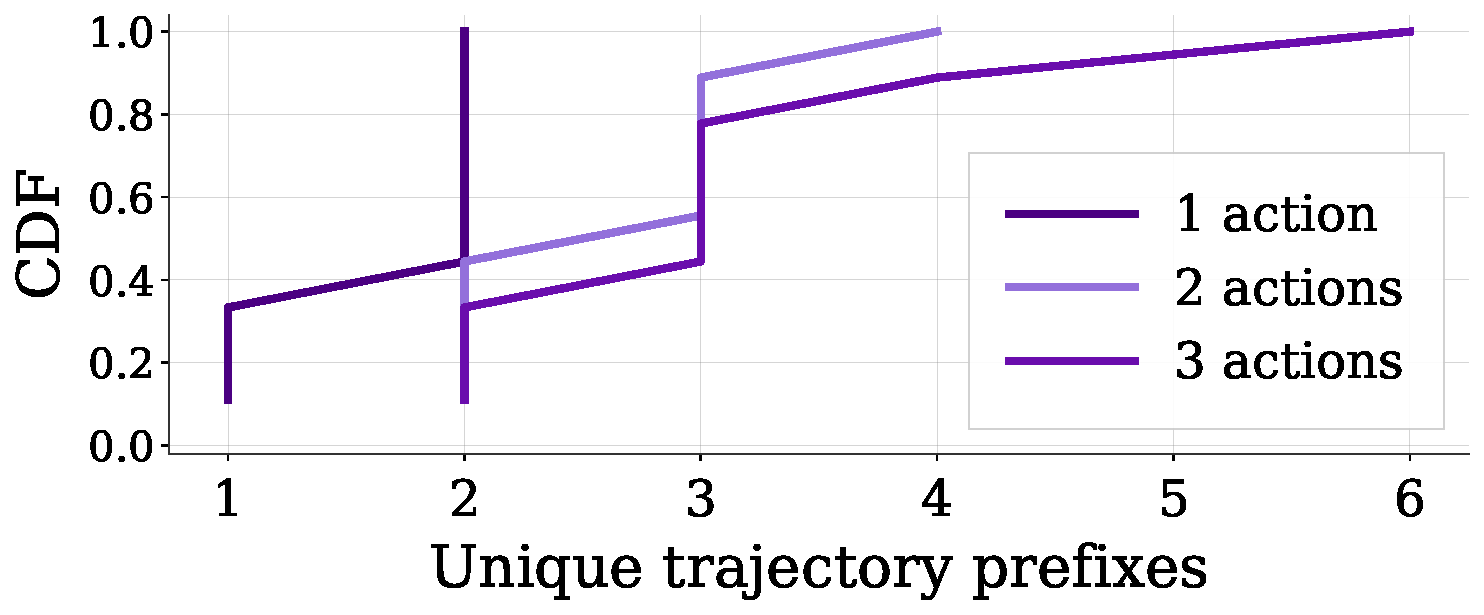
\includegraphics[width=0.99\columnwidth]{figures/trajectory_prefixes_cdf.pdf}
    % \vspace{-2em}
    \tightcaption{Distribution of the number of unique action-type prefixes across tasks on a site, for the first 1, 2, and 3 actions of each task. Prefixes consider action types (e.g., click, type), ignoring parameters like element identifiers or extracted content.}
    \label{fig:trajectory-prefixes}
\end{figure}

\subsection{Runtime Speculation}
\label{sec:design:runtime}
% The runtime cascade begins when a task arrives. \sys{} matches
% the task text against the profile's templates and slot-fills
% from the task description: ``find the abstract of arXiv paper
% 2401.12345'' matches the direct-identifier template with slot
% \texttt{2401.12345}; ``find the cheapest blue headphones on
% % Amazon'' matches the search-query template.\sn{How robust/general is this matching? strict string match? regex matching? LLM-based matching? } If no template
% matches, the task routes directly to the default ReAct agent. If
% a template matches, \sys{} determines the minimum resources the
% task requires from the profile, executes, verifies the output,
% and escalates resources on rejection.

%\begin{sloppypar}
When a task arrives, \sys matches the task against the profile's typed templates through a hybrid process: a lightweight LLM performs intent classification to select a candidate template class (e.g., direct identifier lookup, filtered search, paginated retrieval), while profile-defined regex constraints and parameter validators ground extracted slot values into site-valid parameters. The LLM thus handles semantic interpretation while typed parameter constraints enforce structural validity and prevent free-form generation. For example, ``find the abstract of arXiv paper 2401.12345'' matches the direct-identifier template with slot \texttt{2401.12345}, while ``find the cheapest blue headphones on Amazon'' matches the filtered search template with query, sort-order, and optional price slots. This combination is more robust than strict string or regex-only matching, and more reliable and cheaper than unconstrained frontier-model trajectory planning.
If no template matches with sufficient confidence, the task routes directly to the default ReAct agent. Otherwise, \sys determines the minimum resources the task requires from the profile, executes the speculative fast path, verifies the output, and escalates resources on rejection.
%\end{sloppypar}

%Runtime speculation cascade begins when a task arrives. \sys{} first matches the task text against the profile’s typed templates and extracts candidate slot values from the task description. The matching process is hybrid rather than purely symbolic: lightweight LLM-based intent classification selects candidate template classes (e.g., direct identifier lookup, filtered search, paginated retrieval), while profile-defined regex constraints and parameter validators ground the extracted slots into site-valid parameter values. For example, find the abstract of arXiv paper 2401.12345'' matches the direct-identifier template with slot \texttt{2401.12345}, while find the cheapest blue headphones on Amazon'' matches the filtered search-query template with slots corresponding to the query string, sort order, and optional price constraints. The LLM therefore performs semantic interpretation of the task, while the profile’s typed parameter constraints enforce structural validity and prevent unconstrained free-form generation. This combination makes matching substantially more robust than strict string matching or regex-only approaches while remaining more reliable and lower-cost than unconstrained frontier-model trajectory planning.

%If no template matches with sufficient confidence, the task routes directly to the default ReAct agent. Otherwise, \sys{} determines the minimum resources the task requires from the profile, executes the speculative fast path, verifies the output, and escalates resources on rejection.


Resource determination operates along three axes that govern how
a task is executed:
\begin{sloppypar}
\begin{itemize}
    \item \textbf{Page acquisition.} Either direct URL fetch
    (the page is reachable by URL synthesis from the profile
    template) or multi-step navigation (the ReAct loop). The
    profile dictates which is applicable for the task class.
    \item \textbf{Page rendering.} Either HTTP-only fetch or
    browser-driven rendering. The profile encodes which pages
    on a site require browser rendering (client-side JavaScript,
    authenticated state); pages flagged as HTTP-reachable use
    HTTP, the rest use the browser.
    \item \textbf{Reasoning model.} Either a non-frontier
    extraction model or a frontier model. The profile's answer
    schema and the cleaned page content together determine
    whether the non-frontier model can extract reliably; otherwise a frontier model is used.
\end{itemize}
\end{sloppypar}

The cheapest combination the profile justifies is tried first.
On verification failure, \sys{} escalates the axis the verifier
signals is at fault: a rejection on a missing-but-expected field
escalates the reasoning model, a rejection on an empty or blocked
page escalates rendering to the browser, and persistent failure
escalates page acquisition to full ReAct. Escalation is not a
strict hierarchy; different tasks exercise different axes. Some
need browser rendering with a non-frontier model, others need
HTTP with a frontier model, and many need only the cheapest
combination on all three. The verifier is the feedback signal
that drives axis-specific escalation rather than blind progression
through fixed tiers.

%Two empirical observations about the web domain motivate the
%verifier and warm-start design. First, trajectories on a single
%site share structural prefixes even when their task-specific
%tails differ, so a cheap path that fails has typically still
%completed real navigational progress that recovery can inherit.
%Second, verification on read-only tasks is structurally cheap:
%a site's templates, a task, and a short summary of where the
%agent landed carry enough evidence to confirm or reject without
%re-traversing the page. The first motivates the warm-start
%cascade, which inherits the URL the failed attempt reached. The
%second makes a fast-path verifier viable within the cost
%envelope the cheap path establishes.

This feedback-driven escalation rests on two empirical properties of purpose-built websites: trajectory prefixes are highly predictable, making failed speculation useful, and verification is highly constrained, making it cheap to evaluate.

%\para{Trajectories share structural prefixes.} Because sites are purpose-built around consistent interaction patterns (\S\ref{sec:opp}), trajectories on a site share a structural prefix even when their task-specific tails differ. This split matches Accio's offline/online structure: the shared prefix is what the offline profile encodes, while task-specific tails are what runtime synthesis instantiates. The cheap execution path is therefore well-suited to the structural prefix and progressively less well-suited as trajectories enter their task-specific tails. Even when the cheap path eventually fails, it has typically completed real navigational progress that can be inherited by recovery.

\para{Trajectories share structural prefixes.} On purpose-built sites, queries with different end goals typically begin with identical navigational steps (e.g., search, filter, sort) (Figure \ref{fig:trajectory-prefixes}). This split aligns with \sys{}'s offline/online design: the offline profile captures the shared prefix, while runtime synthesis executes the task-specific tail. Because the speculative fast path excels at navigating these common prefixes, even a trajectory that ultimately fails usually reaches a useful intermediate URL. A more expensive recovery policy can then inherit this progress rather than starting from scratch.


%Although different tasks produce different specific trajectories (different URLs, different parameters, different content), those trajectories share a structural prefix because sites are purpose-built around consistent interaction patterns. Two Amazon shopping tasks visit different specific product pages but both pass through the same sequence of action types: search, navigate from results, land on a product page. Two arXiv tasks fetch different specific papers, both via the same identifier-based URL construction. Two GitHub tasks visit different repositories, both resolved through the same \texttt{owner/repo} pattern. The shared structure is what the offline profile encodes; the task-specific tails (which product, which paper, which repository) are what runtime synthesis instantiates. The cheap execution path is therefore well-suited to the structural prefix and progressively less well-suited as trajectories enter their task-specific tails. Even when the cheap path eventually fails, it has typically completed real navigational progress before failing, and that progress can be inherited by recovery.

%\para{Verification is structurally cheap.}
%Two properties keep verification cheap. First, the verifier has a strong prior: the site supplies the set of structurally valid trajectory templates, and the task selects which one applies. A verifier presented with 'find my last order' and a state summary placing the agent on the orders page recognizes alignment; the same verifier with 'find the cheapest blue headphones' and the same state summary recognizes deviation. Second, web state and answers compress cleanly enough to verify from a few sentences plus a URL. We empirically verify this cheapness against a frontier-model verifier baseline in \S\ref{sev:eval}.

\para{Verification is structurally cheap.}
Checking whether a read-only trajectory succeeded is inexpensive for two reasons. First, the site's profile provides a strong structural prior: it defines the valid navigation templates, reducing the verification problem to checking alignment between the expected task structure and the current state. Second, web state compresses well: a short textual summary of the retrieved content, combined with the URL, is usually sufficient to confirm or reject the outcome without relying on expensive full-page DOM processing. We empirically validate this efficiency against a frontier-model verifier in \S\ref{sev:eval}.



%\todo{How do we show verification is cheap? WE can compare structural verification with cheap model vs frontier model naive verification} Two properties keep verification cheap. First, given a site and a task, the verifier has a strong prior: the site supplies the set of structurally valid trajectory templates, and the task selects which template applies. A verifier presented with the task ``find my last order'' and a state summary placing the agent on the orders page recognizes alignment; the same verifier with ``find the cheapest blue headphones'' and the same state summary recognizes deviation. Second, web state and web answers compress cleanly: a few sentences of state summary, a URL, and a candidate answer carry enough evidence to confirm or reject without the full page.


\para{HTML cleaning is a prerequisite.}
As shown in \S\ref{sec:background}, non-frontier models perform substantially better when input is condensed to task-relevant regions. \sys therefore filters each fetched page against the profile's answer schema before extraction or verification, retaining content matching expected response structure (titles, prices, abstracts) and discarding the rest. This serves both stages: the extraction model operates on focused evidence, and the verifier receives a smaller input that keeps its cost cheap.


%As shown in §\ref{sec:background}, non-frontier models perform substantially better when the input HTML is condensed to the task-relevant regions and unnecessary page scaffolding is removed. Real web pages contain large amounts of human-facing but task-irrelevant content: navigation menus, recommendation panels, advertisements, animated widgets, related-content sidebars, and footer links. \sys therefore filters each fetched page against the profile’s answer schema before invoking either the extraction model or the semantic verifier. The filter retains content matching the expected response structure, such as titles, prices, abstracts, ratings, or metadata fields, and discards the surrounding page chrome. This condensed representation lets the non-frontier model operate on focused evidence rather than a noisy full DOM, improving extraction reliability while also reducing verifier input size and cost. Without cleaning, the small model would face the same full-page ambiguity that causes lightweight ReAct substitutions to fail; with cleaning, it receives an input whose complexity better matches its capabilities.

\para{Two-stage verification.}
The verifier spans the failure-mode spectrum identified in C2 at
low marginal cost. The first stage is a near-zero-cost schema
check: the candidate answer must be non-empty, type-compatible
with the task, and within the expected value range encoded in
the profile. This stage catches obvious failures (bot-detection
pages, empty results, type-mismatched answers) without
an LLM. The second stage runs only on answers that pass the
schema check: a non-frontier semantic judge presented with a
compressed state summary (task description, current URL, cleaned
page summary, candidate answer) decides whether the trajectory
is consistent with the task. Both stages reuse machinery already
provisioned for the fast path. Crucially, the verifier must
be cheap: if verifying the fast path required a frontier
model over the full DOM, the cost of verification would negate
the savings of the fast path. The two-stage design keeps
verification within the per-task cost envelope the fast path
establishes and false positives waste only a retry.

\para{Warm-start cascade.}
On verification rejection, \sys{} retries the task with
escalated resources, inheriting the URL the prior attempt
reached. The cascade preserves the navigational progress the
cheaper attempt made correctly (per the prefix-sharing
observation above), discarding only what the verifier rejected.
Only the URL is propagated: the rejected attempt's extracted
answer and reasoning trace are not, and the escalated attempt
performs its own independent reasoning from the warm-start page.
The URL itself is monotone progress in the sense that escalation
never starts from a position worse than where the cheaper attempt
reached. ReAct's per-step adaptation is designed to handle
exactly this kind of recovery, so a default-agent
cascade resuming at a warm-start URL behaves as a normal ReAct
trajectory starting from that URL rather than from the task's
initial page.

Incorrect warm starts, although infrequent, are also relatively inexpensive to recover from. Because intermediate navigation on read-only tasks is scaffolding rather than load-bearing reasoning (\S\ref{sec:background}), landing on the wrong URL does not require undoing irreversible state mutations or reasoning dependencies -- the agent only needs to redirect navigation toward a different destination page. ReAct's iterative-recovery design handles this naturally, so recovering from an incorrect warm-start URL behaves like any other mid-trajectory navigation adjustment. %In practice, this makes speculative warm starts robust even when the initial trajectory guess is imperfect.

\subsection{Query Support and Deployment Discussion}

\begin{sloppypar}
\sys targets read-dominant web workloads, including search, comparison, structured extraction, and exploratory navigation. These workloads constitute a large fraction of modern  deployments, including retrieval-augmented assistants, deep-research systems, shopping assistants, and enterprise information-gathering pipelines. In these settings, execution cost is dominated not by the final interaction itself, but by exploratory navigation and repeated frontier-model inference over intermediate pages.
\end{sloppypar}

Stateful actions such as purchases, form submissions, or account modifications impose substantially stronger correctness and safety requirements because incorrect execution may produce irreversible side effects. Supporting such workflows robustly requires infrastructure for authentication management, transactional safety, and side-effect validation, which we leave to future work. Nonetheless, workflows that ultimately perform state mutations are typically dominated by long read-only prefixes involving search, filtering, comparison, and navigation. \sys accelerates this expensive exploratory phase while delegating irreversible transactional actions to conventional browser-agent execution.

A second design goal is broad applicability across arbitrarily-worded tasks and heterogeneous websites. Rather than hardcoding a fixed collection of domains or task schemas, lightweight language models map free-form task descriptions onto profile-encoded patterns through typed template matching and parameter extraction. As more sites are profiled, the system naturally expands coverage without requiring changes to the core runtime architecture.

\begin{comment}
\sys{} is designed primarily for \emph{read-only} web tasks:
queries whose goal is to retrieve, compare, summarize, or extract
information from the web without mutating persistent site state.
Examples include product retrieval, literature search, repository
lookup, comparison shopping, structured extraction, and
multi-page information gathering. This focus is intentional.
Read-only browsing comprises a substantial fraction of practical
web-agent workloads: most user tasks involve navigating,
searching, filtering, and exploring the web rather than executing
state-changing actions. Retrieval-augmented assistants,
deep-research systems, shopping assistants, and enterprise search
pipelines are dominated by these read-only interactions, where
the primary cost comes from exploratory navigation and repeated
frontier-model inference rather than from the final interaction
itself.

Accordingly, our evaluation focuses exclusively on read-only
benchmarks and retrieval-oriented tasks. We do not evaluate
stateful actions such as adding items to carts, submitting forms,
creating forum posts, modifying account settings, or completing
transactions. Supporting such state-mutating tasks robustly
requires substantially more infrastructure than speculative
retrieval alone, including reliable request synthesis,
authentication handling, anti-CSRF protections, rollback safety,
and correctness guarantees for side-effecting actions. We leave
these extensions to future work. Importantly, however, the core
ideas behind \sys{} remain useful even in partially stateful
workflows. Many stateful tasks contain large read-only prefixes:
searching for products before adding one to a cart, locating a
discussion thread before posting, or navigating to a reservation
page before checkout. \sys{} can still accelerate these workflows
by cheaply traversing the exploratory portion of the trajectory,
reducing browser interaction and frontier-model usage up to the
point where the stateful action must actually occur. In effect,
the system can compress the expensive navigational scaffolding
surrounding stateful actions even when it cannot yet execute the
mutation itself end-to-end.

A second design goal of \sys{} is broad applicability across
arbitrarily-worded tasks and heterogeneous websites. The system is
not limited to a fixed collection of hardcoded domains or narrow
task schemas. Instead, offline profiling constructs reusable site
profiles that capture search behavior, URL patterns, rendering
requirements, and retrieval conventions specialized to each site.
At runtime, lightweight language models map free-form task
descriptions onto these structural patterns through typed
template matching and constrained parameter extraction. The
resulting design allows \sys{} to generalize across diverse
retrieval tasks while still exploiting the strong structural
regularities present within purpose-built websites. As more sites
are profiled, the system naturally expands its coverage of common
navigation patterns and query types without requiring changes to
the core runtime architecture.
\end{comment}
